\subsection{Project planning}
The Project planning sequence diagram illustrated in figure \ref{3img:[sequence]project_planning} provides the messages exchanged in order find the best organization to istantiate a project. In particular are analyzed several aspects concerning the resources management and above all the Human Resources considered by AllSpark as first fit needing.

A relevant contribution to the plan is the Analyst's work who is charged to correct schedule the working load on the available resources. In this duty is supported by the Project Manager that may brings useful ideas thanking his open minded experience.

As each important action in the Company, the proposal should be approved by the CEO once the expected budget has been calculated. When the confirm reach the Project Manager, the project can finally start.

\begin{figure}[H]
\begin{centering}
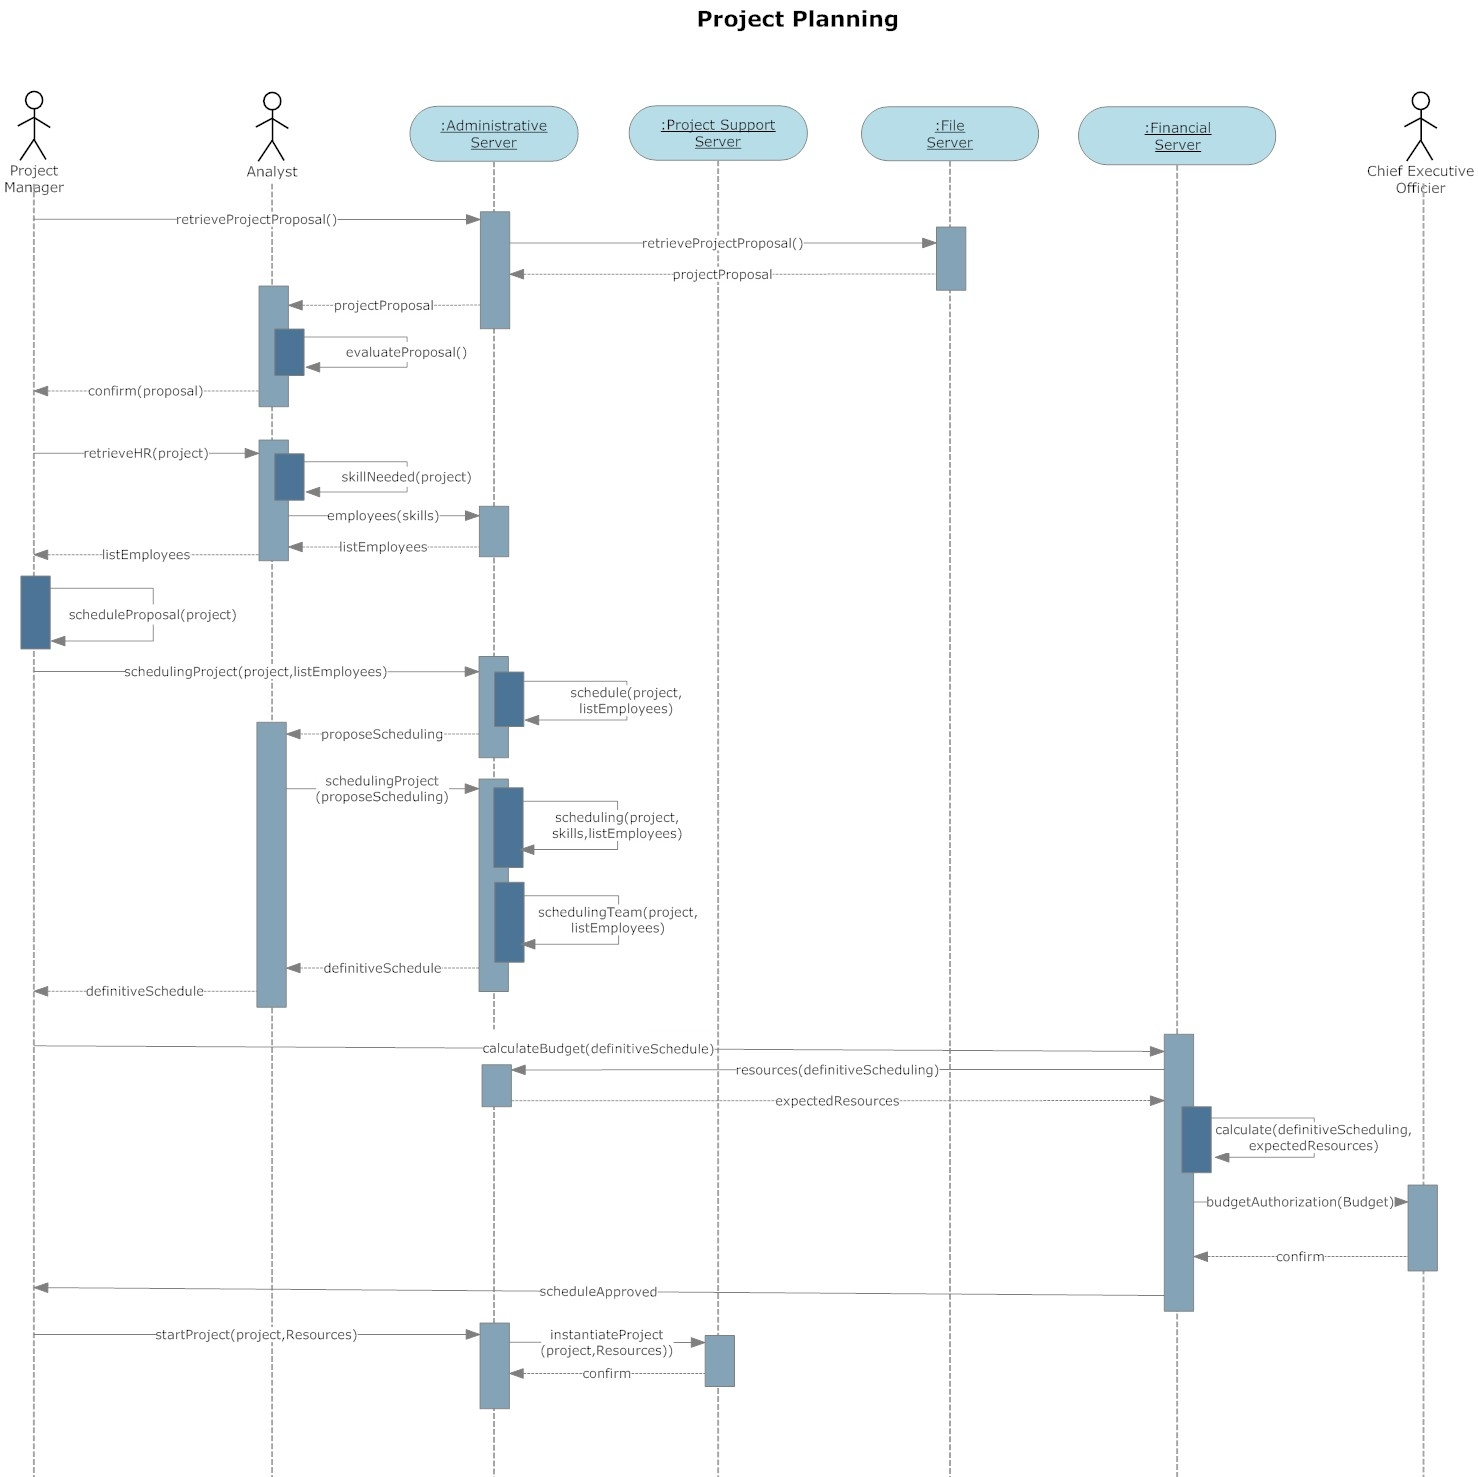
\includegraphics[scale=0.30,angle=90]{assign3/sdraw/imgs/project_planning.jpg}
\caption{Project planning sequence diagram.}
\label{3img:[sequence]project_planning}
\end{centering}
\end{figure}


\subsection{Checking work}
The checking work activity figured in \ref{3img:[sequence]checking} aims to monitor the project status with respect the foreseen scheduling. Once the information are retrieved by the Analyst, a ``case-study`` session with the Project Manager may reveals some problem on Project conducting. With high probability some settlement changes are needed to improve the efficiency in the project lifecycle or to front some unforseen events.

Once the CEO is knowing the status and the changes proposed, the Analyst provide to address the correct directives to the running project.

\begin{figure}[H]
\begin{centering}
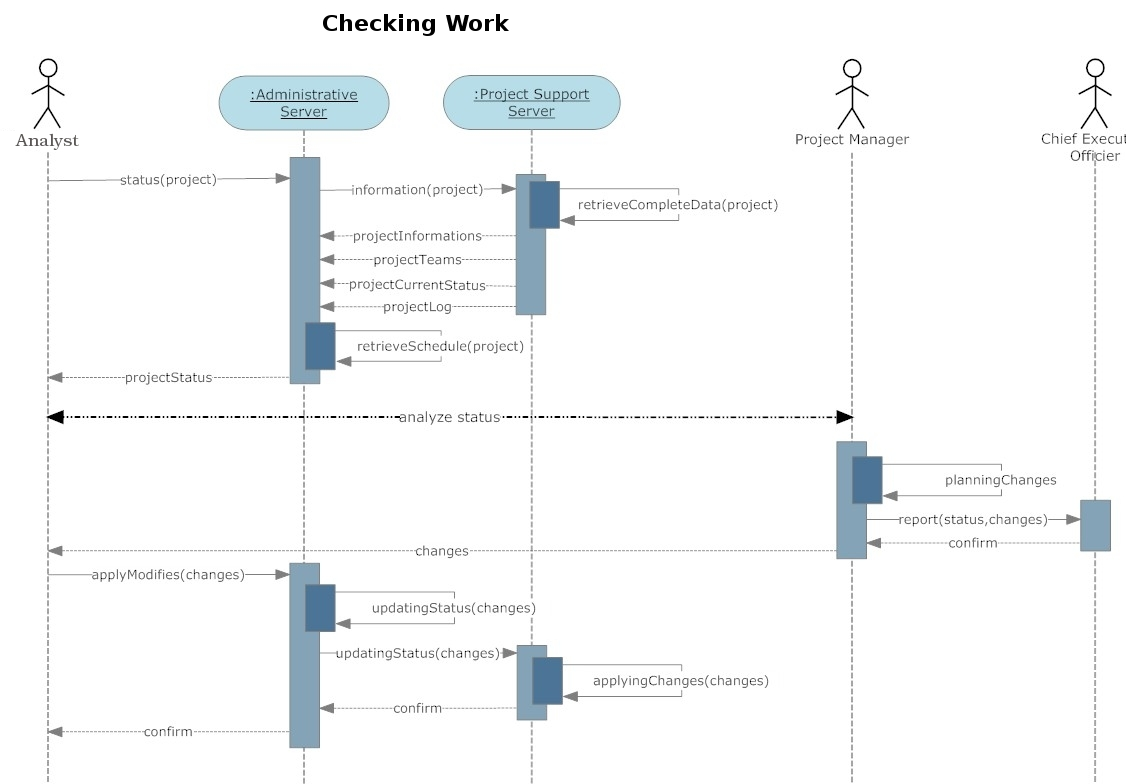
\includegraphics[scale=0.35]{assign3/sdraw/imgs/checking.jpg}
\caption{Checking work sequence diagram.}
\label{3img:[sequence]checking}
\end{centering}
\end{figure}

\subsection{Team monitoring}
\begin{figure}[H]
\begin{centering}
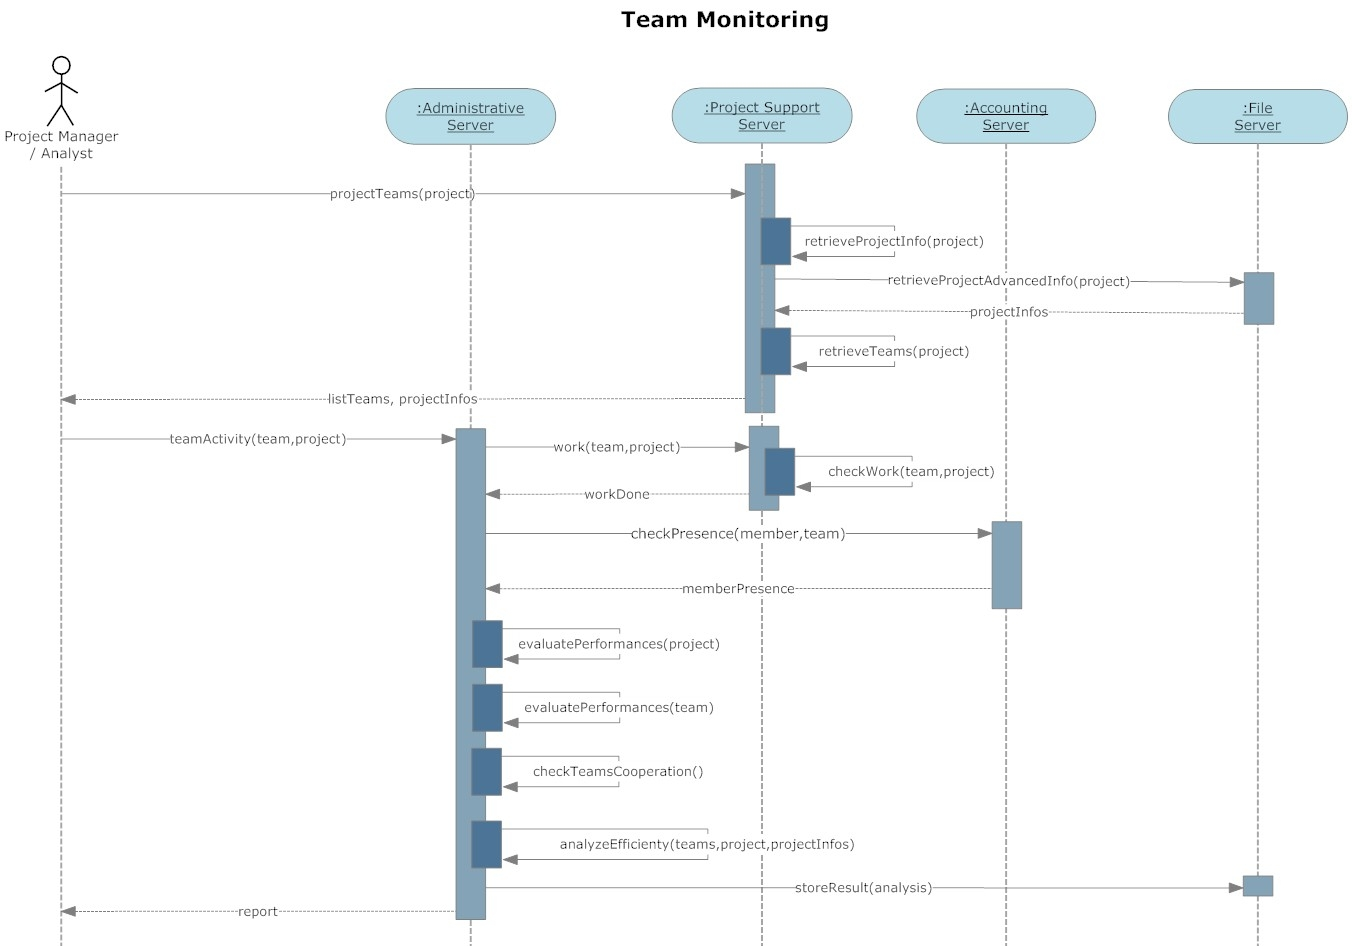
\includegraphics[scale=0.40,angle=90]{assign3/sdraw/imgs/team_monitoring.jpg}
\caption{Team monitoring sequence diagram.}
\label{3img:[sequence]team_monitoring}
\end{centering}
\end{figure}